%%%%%%%%%%%%%%%%%%%%%%%%%%%%%%%%%%%%%%%%%%%%%%%%%%%%%%%%%%%%%%%%%%%%%%%%%%%%%%%%%%%%%%%%%%%%%%%%
%
% CS484 Written Question Template
%
% Acknowledgements:
% The original code is written by Prof. James Tompkin (james_tompkin@brown.edu).
% The second version is revised by Prof. Min H. Kim (minhkim@kaist.ac.kr).
%
% This is a LaTeX document. LaTeX is a markup language for producing 
% documents. Your task is to fill out this document, then to compile 
% it into a PDF document. 
%
% 
% TO COMPILE:
% > pdflatex thisfile.tex
%
% If you do not have LaTeX and need a LaTeX distribution:
% - Personal laptops (all common OS): www.latex-project.org/get/
% - We recommend latex compiler miktex (https://miktex.org/) for windows,
%   macTex (http://www.tug.org/mactex/) for macOS users.
%   And TeXstudio(http://www.texstudio.org/) for latex editor.
%   You should install both compiler and editor for editing latex.
%   The another option is Overleaf (https://www.overleaf.com/) which is 
%   an online latex editor.
%
% If you need help with LaTeX, please come to office hours. 
% Or, there is plenty of help online:
% https://en.wikibooks.org/wiki/LaTeX
%
% Good luck!
% Min and the CS484 staff
%
%%%%%%%%%%%%%%%%%%%%%%%%%%%%%%%%%%%%%%%%%%%%%%%%%%%%%%%%%%%%%%%%%%%%%%%%%%%%%%%%%%%%%%%%%%%%%%%%
%
% How to include two graphics on the same line:
% 
% \includegraphics[width=0.49\linewidth]{yourgraphic1.png}
% \includegraphics[width=0.49\linewidth]{yourgraphic2.png}
%
% How to include equations:
%
% \begin{equation}
% y = mx+c
% \end{equation}
% 
%%%%%%%%%%%%%%%%%%%%%%%%%%%%%%%%%%%%%%%%%%%%%%%%%%%%%%%%%%%%%%%%%%%%%%%%%%%%%%%%%%%%%%%%%%%%%%%%

\documentclass[11pt]{article}

\usepackage[english]{babel}
\usepackage[utf8]{inputenc}
\usepackage[colorlinks = true,
            linkcolor = blue,
            urlcolor  = blue]{hyperref}
\usepackage[a4paper,margin=1.5in]{geometry}
\usepackage{stackengine,graphicx}
\usepackage{fancyhdr}
\setlength{\headheight}{15pt}
\usepackage{microtype}
\usepackage{times}

% From https://ctan.org/pkg/matlab-prettifier
\usepackage[numbered,framed]{matlab-prettifier}

\frenchspacing
\setlength{\parindent}{0cm} % Default is 15pt.
\setlength{\parskip}{0.3cm plus1mm minus1mm}

\pagestyle{fancy}
\fancyhf{}
\lhead{Homework 4 Questions}
\rhead{CS 484}
\rfoot{\thepage}

\date{}

\title{\vspace{-1cm}Homework 4 Questions}


\begin{document}
\maketitle
\vspace{-3cm}
\thispagestyle{fancy}

\section*{Instructions}
\begin{itemize}
  \item 4 questions.
  \item Write code where appropriate.
  \item Feel free to include images or equations.
  \item Please make this document anonymous.
  \item \textbf{Please use only the space provided and keep the page breaks.} Please do not make new pages, nor remove pages. The document is a template to help grading.
  \item If you really need extra space, please use new pages at the end of the document and refer us to it in your answers.
\end{itemize}

\section*{Questions}

\paragraph{Q1:} Imagine we were tasked with designing a feature point which could match all of the following three pairs of images. Which real world phenomena and camera effects might cause us problems?
Use the MATLAB function \href{https://www.mathworks.com/help/images/ref/corner.html}{$corner$} to investigate. $corner(I,1000)$.

\emph{RISHLibrary} | \emph{Chase} | \emph{LaddObservatory}

%%%%%%%%%%%%%%%%%%%%%%%%%%%%%%%%%%%
\paragraph{A1:} The image for Chase is shaken possibly due to low light conditions. Images for Ladd Observatory contain too much of different objects \emph{e.g.} people. Images for the RISH Library have different color tones. To design a feature point that match all of the three pairs, the conditions of them should be similar. However, in this case the three pairs have different characteristics that it is difficult for a common feature point to match them. This phenomenon is common in the real world, which makes it difficult to make  feature points.
\begin{figure}[h!]
	\centering
	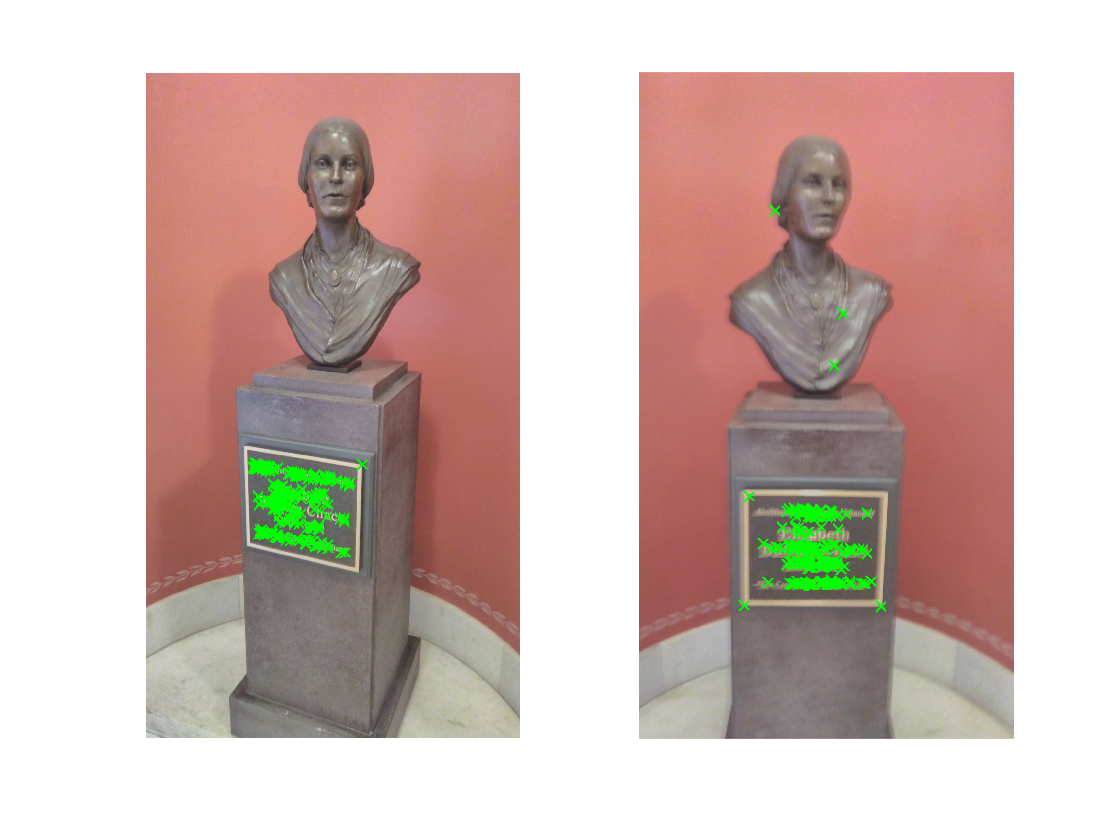
\includegraphics[width=0.3\textwidth]{../code/chase.png}
	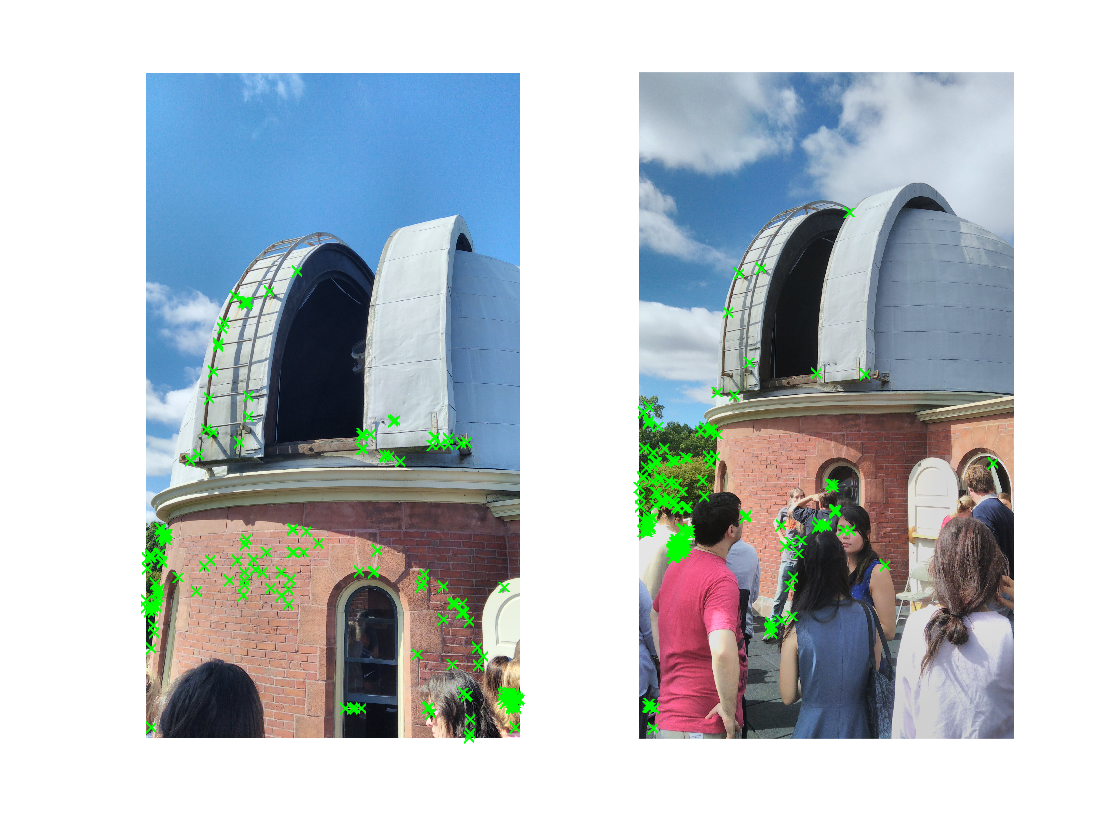
\includegraphics[width=0.3\textwidth]{../code/ladd.png}
	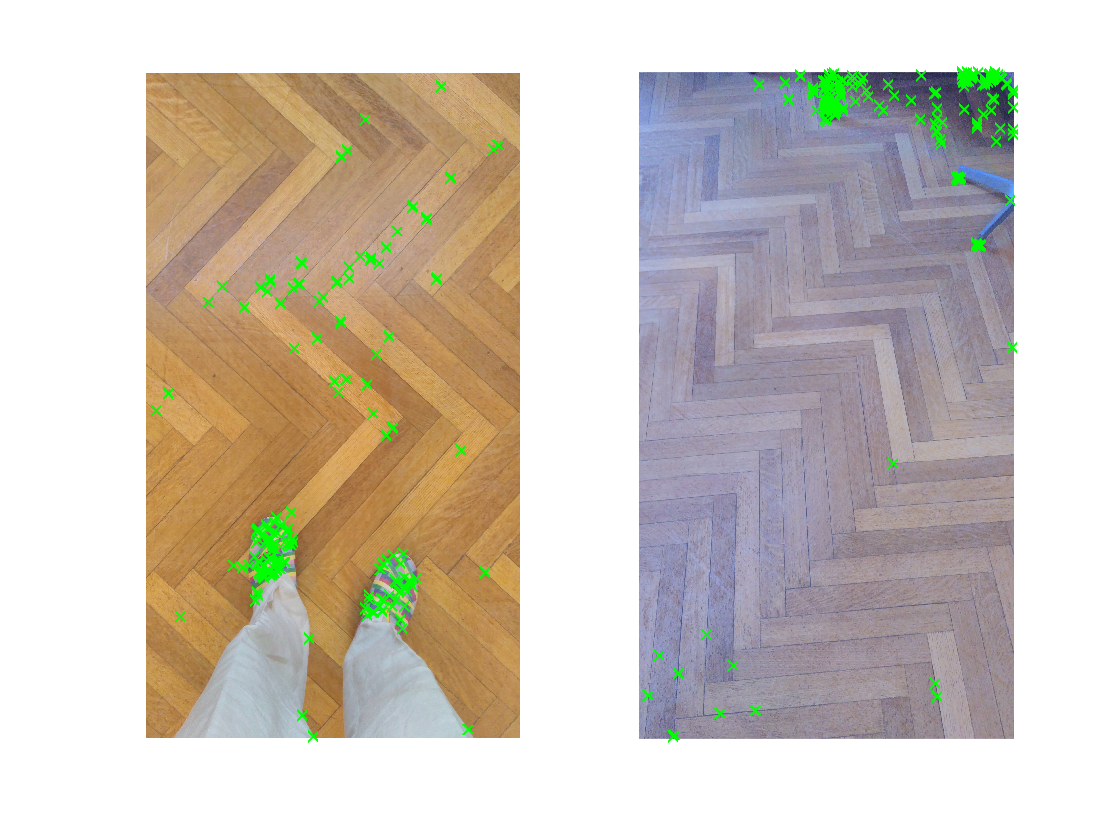
\includegraphics[width=0.3\textwidth]{../code/rish.png}
\end{figure}



%%%%%%%%%%%%%%%%%%%%%%%%%%%%%%%%%%%

% Please leave the pagebreak
\pagebreak
\paragraph{Q2:} In designing our feature point, what characteristics might we wish it to have? Describe the fundamental trade-off between feature point invariance and discriminative power. How should we design for this trade-off?

%%%%%%%%%%%%%%%%%%%%%%%%%%%%%%%%%%%
\paragraph{A2:} Scale and orientation invariance would benefit the feature points. However, this could lead to cases in which a pattern-like image with patterns of different sizes are not distinguished. The patterns of different scale but of same shape would be considered as a same feature even if in fact they are not. A similar issue may arise for patterns of different orientation that are considered as the same. Parameters such as the window size and threshold could be adjusted so that the similar features are distinguished.



%%%%%%%%%%%%%%%%%%%%%%%%%%%%%%%%%%%

% Please leave the pagebreak
\pagebreak
\paragraph{Q3:} In the Harris corner detector, what do the eigenvalues of the `M' second moment matrix represent? Discuss both how they relate to image intensity and how we can interpret them geometrically.

%%%%%%%%%%%%%%%%%%%%%%%%%%%%%%%%%%%
\paragraph{A3:} The eigenvalues represent the axis lengths of the ellipse. The length of the major axis is determined by $\lambda_{min}$ by the formula $\frac{1}{\sqrt{\lambda_{min}}}$. The length of the minor axis is determined by $\lambda_{max}$ by the formula $\frac{1}{\sqrt{\lambda_{max}}}$. The minor axis is the direction of the fastest change in intensity, and the major axis is the direction of the slowest change in intensity.



%%%%%%%%%%%%%%%%%%%%%%%%%%%%%%%%%%%


% Please leave the pagebreak
\pagebreak
\paragraph{Q4:} Explain the difference between the Euclidean distance and the cosine similarity metrics between descriptors. What might their geometric interpretations reveal about when each should be used? Given a distance metric, what is a good method for feature descriptor matching and why?

%%%%%%%%%%%%%%%%%%%%%%%%%%%%%%%%%%%
\paragraph{A4:} The cosine similarity is calculated for $A$ and $B$ by the formula $\frac{\sum{A_iB_i}}{{\sqrt{\sum{A_i^2}}}{\sqrt{\sum{B_i^2}}}}$. The Euclidean distance is calculated by the formula $\sqrt{\sum{(B_i-A_i)}^2}$. The cosine similarity is measured by the angle between the vectors thus the magnitudes of them are not considered. In cases the magnitude of the feature vector is important, cosine similarity should not be used. \emph{L1 norm} or \emph{L2 norm} is used as a distance metric for feature matching of string based descriptors such as \emph{SIFT}, \emph{SURF} and \emph{KAZE}. The \emph{Hamming distance} is used for binary descriptors such as \emph{ORB}, \emph{BRISK}, and \emph{BRIEF}.



%%%%%%%%%%%%%%%%%%%%%%%%%%%%%%%%%%%


% If you really need extra space, uncomment here and use extra pages after the last question.
% Please refer here in your original answer. Thanks!
%\pagebreak
%\paragraph{AX.X Continued:} Your answer continued here.



\end{document}
